\section{Data processing}
\label{process}

\subsection{Aggregation}
\label{aggregate}

% We next describe how the simulations and observations were made to be comparable. Figure \ref{weight} shows the spatial locations of each data source for California.

We will analyze precipitation and temperature over both California and the United States. In each case, we take the climate moodel grid cell locations and create non-overlapping cells, or rectangles, such that each location is roughly in the center of the cell (see Figure \ref{weight}). Then we count the number of locations from the observation product that are contained within each cell. The number of locations within the cells are used to weight the climate simulations (the right plot in Figure \ref{weight} shows which climate simulation locations have non-zero weight). For precipitation, we take a weighted sum and for temperature a weighted average. No weighting is used for the observations. Instead, a straight sum or average of all locations within our region of interest (either California or U.S.) is used. This method places the simulations and the observations on the same scale and yields daily time-series.

\begin{figure}
\begin{center}
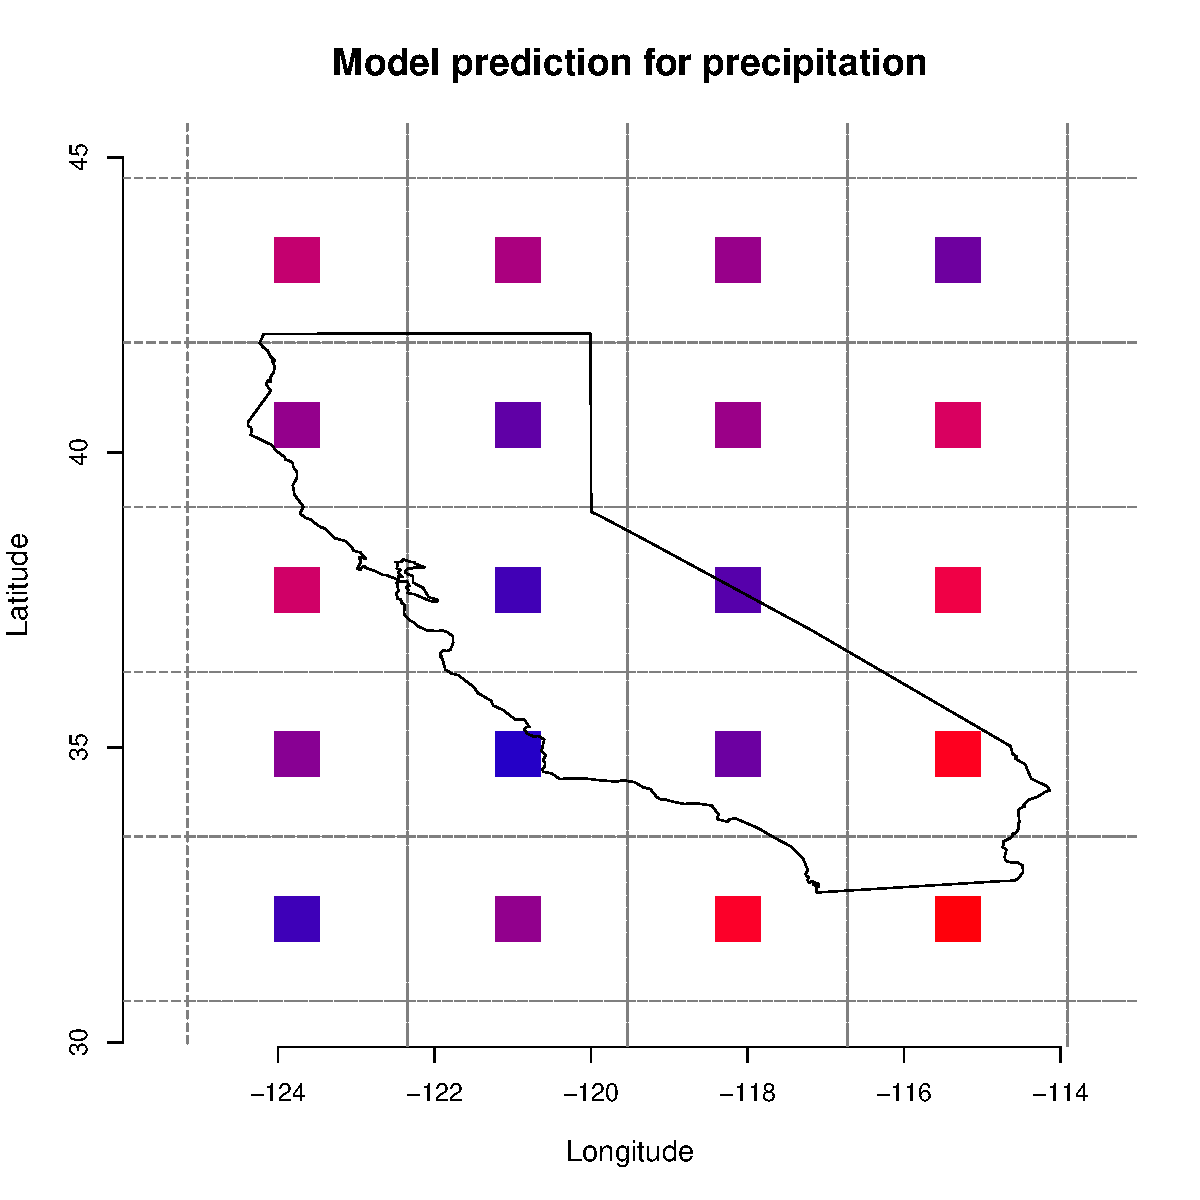
\includegraphics[scale=0.26]{figs/cal_mod_box1.pdf}
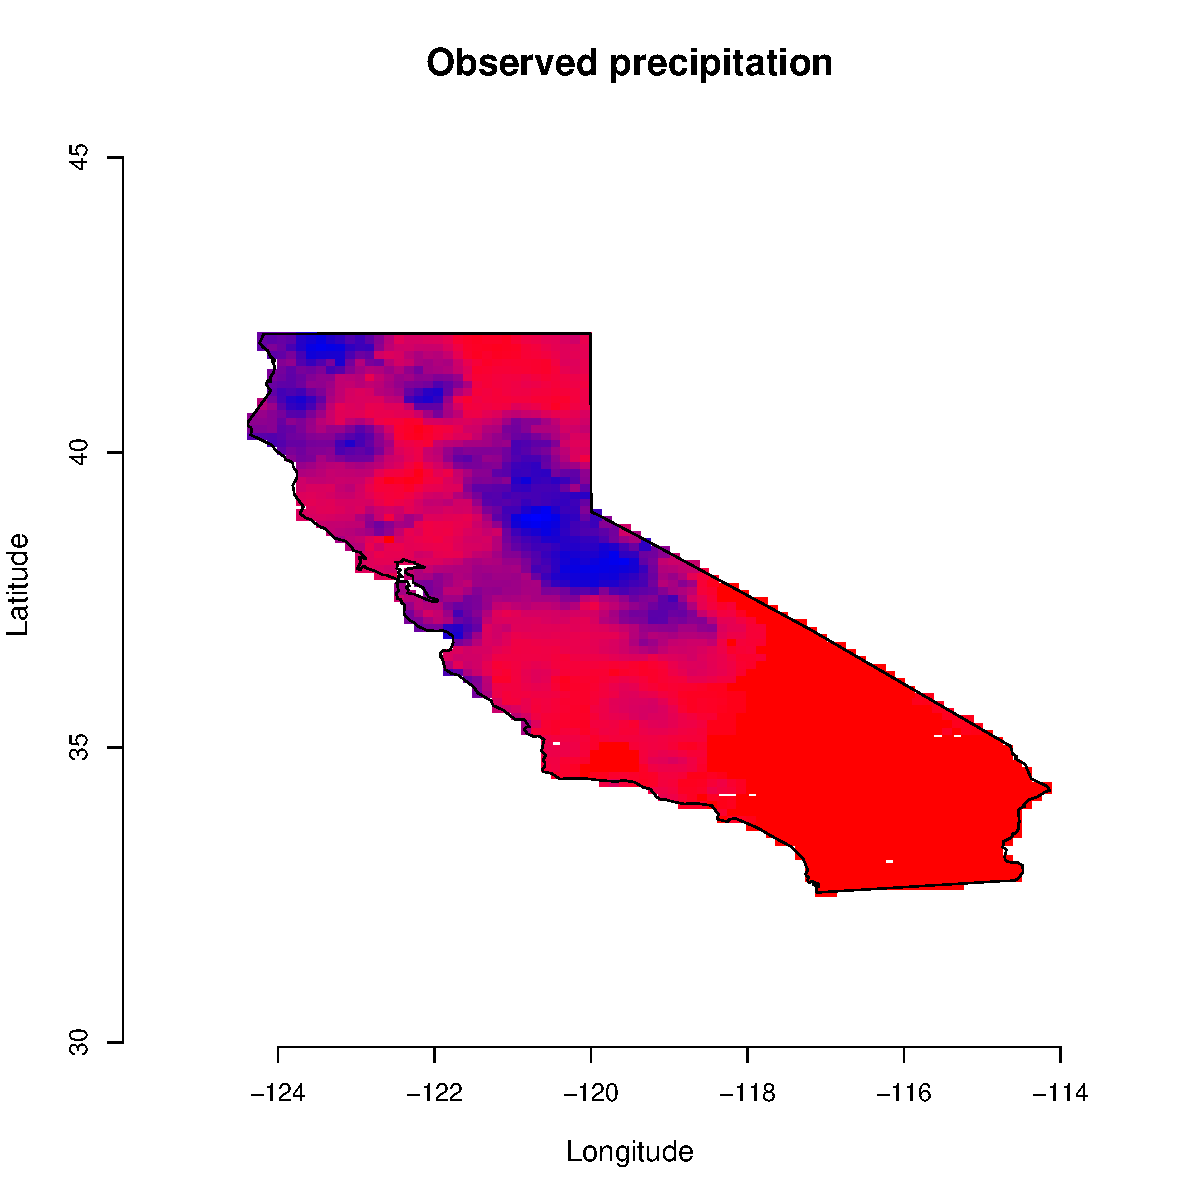
\includegraphics[scale=0.26]{figs/cal_mod_box2.pdf}
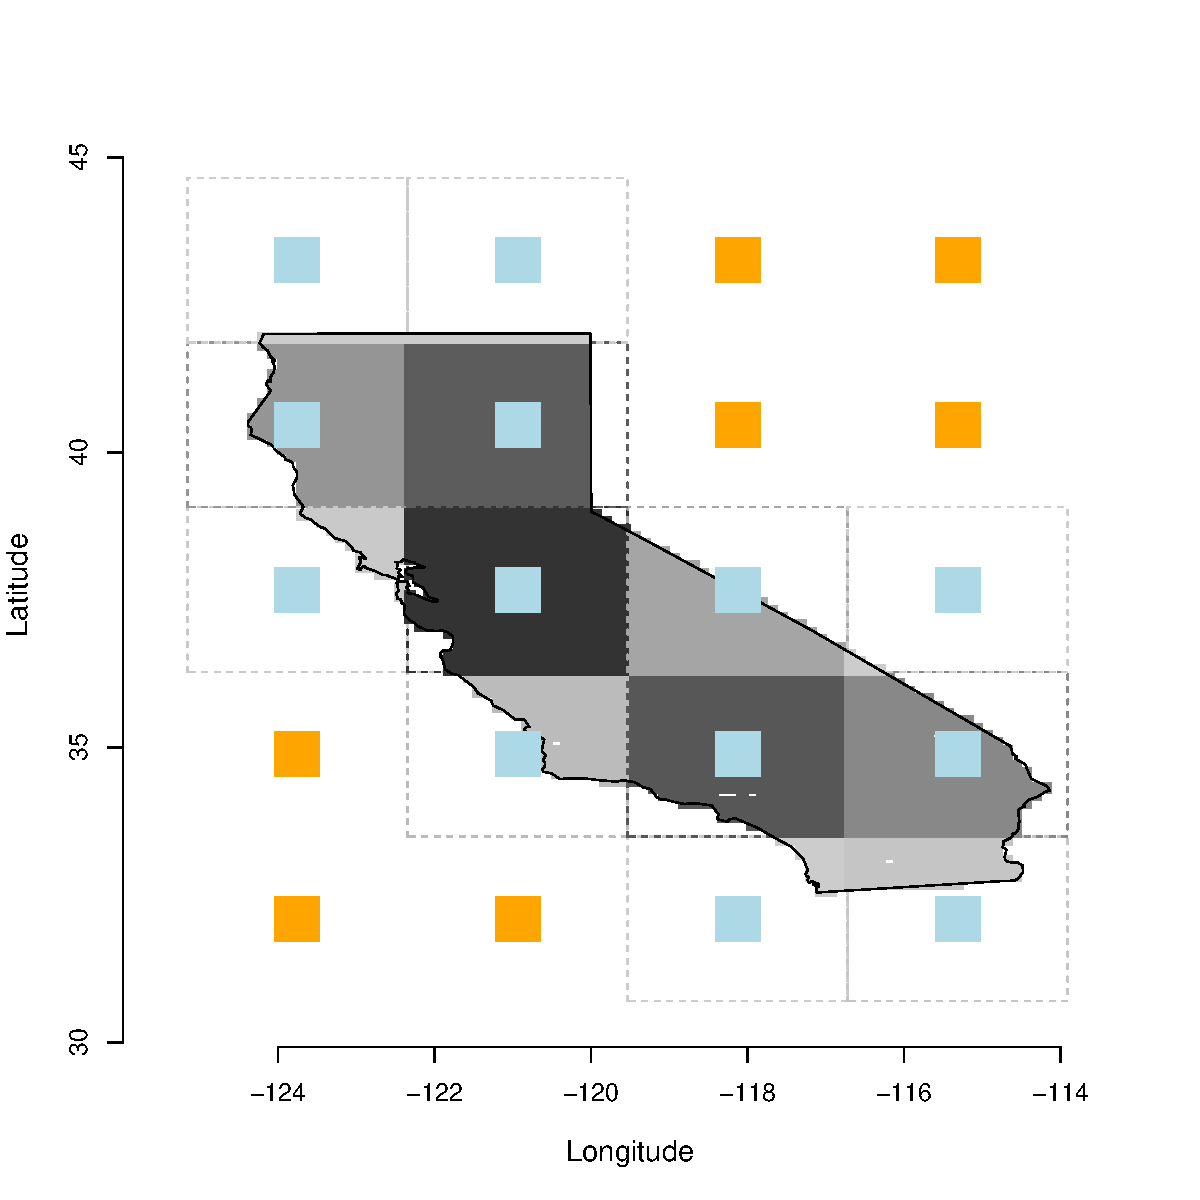
\includegraphics[scale=0.26]{figs/cal_mod_box3.pdf}
\end{center}
\caption{Left: CanCM4 simulation grid cells. Center: Observation locations. Right: method for computing weighted sum or average for CanCM4 to make values comparable with observations; the lighter gray points mean less weight is applied to the climate simulations and the darker gray means more weight. The data shown are from a single day in January.}
\label{weight}
\end{figure}



\subsection{De-trending}
\label{anomaly}

Climate data are often non-stationary series characterized by complicated trends and cycles. As such, these present problems when studying extremes. Since we are interested in the behavior of the extremes, each time-series is ``de-trended'' prior to parameter estimation. This is accomplished through the use of dynamic linear models (DLMs). We will review some basic concepts for DLMs, see \cite{prado2010time} chapter 4 for more details.

\begin{figure}
\begin{center}
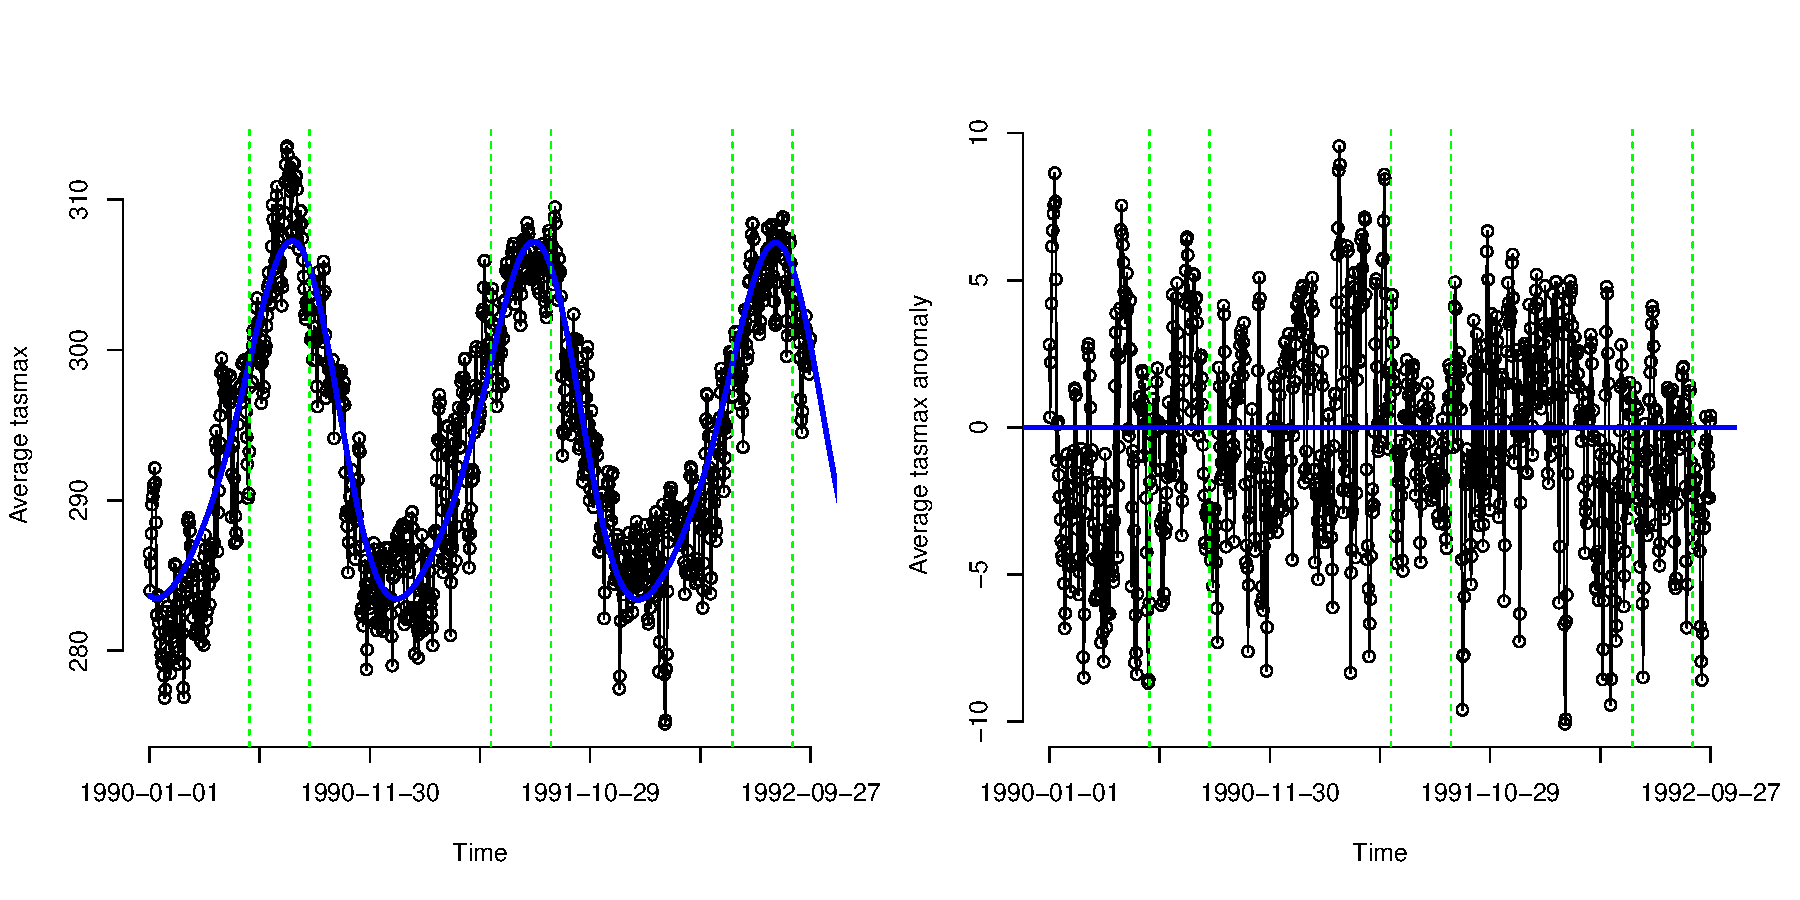
\includegraphics[scale=0.50]{figs/dlm.pdf}
\end{center}
\caption{One of the DLMs used to calculate the anomalies. Shown is one of the decadal replicates of average \texttt{tasmax} in California for about the first two and one-half years of the time-series. The green dashed lines mark the beginning and the end of the summer months.}
\label{dlm_fig}
\end{figure}


A normal DLM is specified by the quadruple $\{\m{F}_t, v_t, \m{G}_t, \m{W}_t\}$ which determine how a univariate time series $y_1,\ldots,y_T$ is modeled over time. We assume
\begin{align}
y_t &= \m{F}_t^\top\m{\theta}_t + \nu_t,~~~~~\nu_t\sim N(0, v_t) \label{dlm_model} \\
\m{\theta}_t &= \m{G}_t\m{\theta}_{t-1}+\m{w}_t~~~~~\m{w}_t\sim N(\m{0}, \m{W}_t) \nonumber
\end{align}
where $\m{\theta}_t$ is the length-$p$ state vector, $\m{F}_t$ is a length $p$ vector of known constants are regressors, $\nu_t$ is obersvation noise, $\m{G}_t$ is the known $p\times p$ state evolution matrix, and $\m{w}_t$ is the state evolution noise. Note that $\nu_s$ and $\m{w}_t$ are independent and mutually independent.

An advantage to model (\ref{dlm_model}) is its capability in yielding a smooth and flexible mean across time. After conditioning on the data up to time $T$, we extrapolate back over time to obtain the posterior distributions $p(\m{\theta}_t|D_T)$ for all $t<T$, which have mean $\m{a}_t$. Using these distributions, and given $\m{F}_t$, the mean of $y_t$ is simply $\m{F}_t^\top\m{a}_t$ (we refer the reader to \cite{prado2010time} for the algorithmic details).

We must omit further details in the interest of space. Our DLM is finalized in the following way. We construct $\m{F}_t$ and $\m{G}_t$ such that the evolution of $\m{\theta}_t$ has annual and semi-annual periods, i.e. the first and second harmonics. Higher harmonics did not seem to make significant contributions in modeling the time-series. A discount factor of $\delta=0.9999$ was chosen, signifying low systematic variance. We assume the prior for $v_t$ is an inverse gamma having sensible shape and scale parameters.

In the end, we are left with the residuals. See Figure \ref{dlm_fig}. The blue line in the left plot is the mean of $y_t$, $\m{F}_t^\top\m{a}_t$, given the whole time series. The interior of the vertical green lines mark the summer months. The right plot is the result of subtracting the observation $y_t$ with the mean from the DLM, which produces a roughly stationary sequence. Thus, in our extreme value analysis we fit our model to the residuals, or anomalies.

For each time-series to be analyzed, we fit a DLM having the characteristics described above to obtain the anomalies. When working within a specific season, either winter (December, January, February) or summer (June, July, August), we concatenate across years to form a single time series of seasonal anoamlies. So, for example in winter, 28 February is followed immediately by 1 December.
